% ----------------------------------------------------------------------
%
%        Vorlage für Abschlussarbeiten am Lehrstuhl Informatik XII
%
%                   http://ls12-www.cs.uni-dortmund.de
%
%   Für Fragen und Anregungen zur Vorlage: info@ls12.cs.uni-dortmund.de
%
%   Stand: 03.09.2013
%
% ----------------------------------------------------------------------

\RequirePackage{ifthen}

\newcommand \type{Fachprojekt Report}
\newcommand \Autor{Lukas B{\"u}nger \\ Thilaksan Kodeeswaran\\ Dilsan Mahadeva}
\newcommand \submissiondate{30.09.2020}
\newcommand \thesistitle{Interactive Real-Time Gaming}
\newcommand \firstsupervisor{Prof.~Dr. Jian-Jia Chen}
\newcommand \secondsupervisor{M.Sc. Junjie Shi}
\newcommand \ErstLehrstuhl{Lehrstuhl Informatik 12 (Eingebettete Systeme) \\ \url{http://ls12-www.cs.tu-dortmund.de}}
\newcommand \ZweitLehrstuhl{}

\RequirePackage{ifpdf} \ifpdf
  \pdfoutput=1
  \pdftrue
  \message{pdfLaTeX}
  \documentclass[pdftex,11pt,a4paper,twoside,ngerman]{scrbook}
  \usepackage{float}
  \usepackage[pdftex]{thumbpdf}
  \usepackage[pdftex]{graphicx}
  \usepackage[pdftex]{hyperref}
  \usepackage{pdfpages}
  \pdfoutput=1
  \pdfcompresslevel=9
  \DeclareGraphicsExtensions{.pdf,.jpg,.png}
\else
  \pdffalse
  \message{LaTeX}
  \documentclass[dvips,11pt,a4paper,twoside,ngerman]{scrbook}
  \usepackage{float}
  \usepackage{graphicx}
  \usepackage{epsf}
  \usepackage[dvips]{hyperref}
  \DeclareGraphicsExtensions{.eps}
\fi

% Informationen fuer pdf-File festlegen
\hypersetup
{
    pdfauthor = {\Autor},
    pdftitle = {\thesistitle},
    pdfsubject = {\type, TU Dortmund, Fakult{\"a}t f{\"u}r Informatik},
    pdfproducer = {LaTeX},
    pdfview = FitV,
    pdfstartview = FitV,
    pdfhighlight = /I,
    pdfborder = 0 0 0,
    colorlinks = false,
    bookmarksopen,
    bookmarksopenlevel = 1,
    bookmarksnumbered = false,
    plainpages = false
}%

% -------------------------------------------------------------------
% Seitenformat anpassen
\usepackage[a4paper,left=3.5cm,right=2.5cm,bottom=3.5cm,top=3cm]{geometry}
\setlength{\headheight}{15pt}

% -------------------------------------------------------------------
% Grafikpakete einbinden
\usepackage{amsmath,amssymb}
\usepackage{flafter}
\usepackage{subfigure}

% -------------------------------------------------------------------
\usepackage{ifthen}

% -------------------------------------------------------------------
\usepackage[absolute,overlay]{textpos}
\setlength{\TPHorizModule}{1mm}
\setlength{\TPVertModule}{\TPHorizModule}
\textblockorigin{0mm}{0mm}
\usepackage{fix-cm}
\usepackage{setspace}
\usepackage{scrhack}

% -------------------------------------------------------------------
% Korrekte Darstellung der Umlaute
% \usepackage[german,ngerman]{babel}
% \usepackage[utf8]{inputenc}
% \usepackage[T1]{fontenc}
% \usepackage{ae,aecompl}

% -------------------------------------------------------------------
% Bibtex deutsch
%\usepackage[numbers,sort,square]{natbib}
%\usepackage{bibgerm}

% -------------------------------------------------------------------
% Anführungszeichen
\usepackage[babel,german=quotes]{csquotes}

% -------------------------------------------------------------------
% URLs
\usepackage{url}

% -------------------------------------------------------------------
% Caption anpassen
\usepackage[margin=0pt,font=small,labelfont=bf]{caption}

% -------------------------------------------------------------------
% Erweitere Tabellen
\usepackage{booktabs}

% -------------------------------------------------------------------
% Eurosymbol
\usepackage{eurosym}

% -------------------------------------------------------------------
% Zeilenabstand einstellen
\renewcommand{\baselinestretch}{1.25}
% Floating-Umgebungen anpassen
\renewcommand{\topfraction}{0.9}
\renewcommand{\bottomfraction}{0.8}

% -------------------------------------------------------------------
% Keine einzelnen Zeilen beim Anfang eines Abschnitts ("Schusterjungen")
\clubpenalty = 10000
% Keine einzelnen Zeilen am Ende eines Abschnitts ("Hurenkinder")
\widowpenalty = 10000 \displaywidowpenalty = 10000
\parindent=0cm

% -------------------------------------------------------------------
% Kopfzeile hinzufuegen
\usepackage{fancyhdr}
\usepackage{extramarks}

\pagestyle{fancy}
\renewcommand{\chaptermark}[1]{\markboth{#1}{}}
\renewcommand{\sectionmark}[1]{\markright{#1}{}}

\fancyhf{}
\fancyhead[LE,RO]{\thepage}
\fancyhead[RE]{\textit{\nouppercase{\leftmark}}}
\fancyhead[LO]{\textit{\nouppercase{\rightmark}}}

\fancypagestyle{plain}{ %
\fancyhf{} % remove everything
\renewcommand{\headrulewidth}{0pt} % remove lines as well
\renewcommand{\footrulewidth}{0pt}} \pagestyle{headings}

% -------------------------------------------------------------------
% Eigene Farben definieren
\usepackage{color}
\definecolor{TUGreen}{rgb}{0.517,0.721,0.094}
\definecolor{TUOrange}{rgb}{1.0,0.7176,0.0}
\definecolor{BrightGray}{gray}{0.9}
\definecolor{DarkGray}{gray}{0.2}
\definecolor{white}{rgb}{1,1,1}
\definecolor{black}{rgb}{0,0,0}
\definecolor{red}{rgb}{1,0,0}

% -------------------------------------------------------------------
% Programm-Listings einbinden und formatieren
\usepackage{listings}

\lstdefinestyle{C++}
{
language=C++,
backgroundcolor=\color{BrightGray},
keywordstyle=\tt\bfseries,  %\color{TUGreen}\bfseries,
commentstyle=\color{DarkGray},
stringstyle=\color{red},
showstringspaces=false,
basicstyle=\small\color{black},
numbers=left,
captionpos=b,
tabsize=4,
breaklines=true
}

% -------------------------------------------------------------------
% Algorithmen
\usepackage[plain,chapter]{algorithm}
\usepackage{algorithmic}

\usepackage{enumerate}

% -------------------------------------------------------------------
% Algorithmen anpassen
\renewcommand{\algorithmicrequire}{\textit{Eingabe:}}
\renewcommand{\algorithmicensure}{\textit{Ausgabe:}}
\floatname{algorithm}{Algorithmus}
\renewcommand{\listalgorithmname}{Algorithmenverzeichnis}
\renewcommand{\algorithmiccomment}[1]{\color{grau}{// #1}}

% -------------------------------------------------------------------
% Theorem-Umgebungen
\usepackage[amsmath,thmmarks]{ntheorem}
\theoremseparator{.}
\theoremstyle{change}
\newtheorem{theorem}{Theorem}[section]
\newtheorem{satz}[theorem]{Satz}
\newtheorem{lemma}[theorem]{Lemma}
\newtheorem{korollar}[theorem]{Korollar}
\newtheorem{proposition}[theorem]{Proposition}
% Ohne Numerierung
\theoremstyle{nonumberplain}
\renewtheorem{theorem*}{Theorem}
\renewtheorem{satz*}{Satz}
\renewtheorem{lemma*}{Lemma}
\renewtheorem{korollar*}{Korollar}
\renewtheorem{proposition*}{Proposition}
% Definitionen mit \upshape
\theorembodyfont{\upshape}
\theoremstyle{change}
\newtheorem{definition}[theorem]{Definition}
\theoremstyle{nonumberplain}
\renewtheorem{definition*}{Definition}
% Kursive Schrift
\theoremheaderfont{\itshape}
\newtheorem{notation}{Notation}
\newtheorem{konvention}{Konvention}
\newtheorem{bezeichnung}{Bezeichnung}
\theoremsymbol{\ensuremath{\Box}}
\newtheorem{beweis}{Beweis}
\theoremsymbol{}
\theoremstyle{change}
\theoremheaderfont{\bfseries}
\newtheorem{bemerkung}[theorem]{Bemerkung}
\newtheorem{beobachtung}[theorem]{Beobachtung}
\newtheorem{beispiel}[theorem]{Beispiel}
\newtheorem{problem}{Problem}
\theoremstyle{nonumberplain}
\renewtheorem{bemerkung*}{Bemerkung}
\renewtheorem{beispiel*}{Beispiel}
\renewtheorem{problem*}{Problem}

% Algorithmen anpassen %
\renewcommand{\algorithmicrequire}{\textit{Eingabe:}}
\renewcommand{\algorithmicensure}{\textit{Ausgabe:}}
\floatname{algorithm}{Algorithmus}
\renewcommand{\listalgorithmname}{Algorithmenverzeichnis}
\renewcommand{\algorithmiccomment}[1]{\color{grau}{// #1}}

% Zeilenabstand einstellen %
\renewcommand{\baselinestretch}{1.25}
% Floating-Umgebungen anpassen %
\renewcommand{\topfraction}{0.9}
\renewcommand{\bottomfraction}{0.8}
% Abkuerzungen richtig formatieren %
\usepackage{xspace}
\newcommand{\vgl}{vgl.\@\xspace} 
\newcommand{\zB}{z.\nolinebreak[4]\hspace{0.125em}\nolinebreak[4]B.\@\xspace}
\newcommand{\bzw}{bzw.\@\xspace}
\newcommand{\dahe}{d.\nolinebreak[4]\hspace{0.125em}h.\nolinebreak[4]\@\xspace}
\newcommand{\etc}{etc.\@\xspace}
\newcommand{\evtl}{evtl.\@\xspace}
\newcommand{\ggf}{ggf.\@\xspace}
\newcommand{\bzgl}{bzgl.\@\xspace}
\newcommand{\so}{s.\nolinebreak[4]\hspace{0.125em}\nolinebreak[4]o.\@\xspace}
\newcommand{\iA}{i.\nolinebreak[4]\hspace{0.125em}\nolinebreak[4]A.\@\xspace}
\newcommand{\sa}{s.\nolinebreak[4]\hspace{0.125em}\nolinebreak[4]a.\@\xspace}
\newcommand{\su}{s.\nolinebreak[4]\hspace{0.125em}\nolinebreak[4]u.\@\xspace}
\newcommand{\ua}{u.\nolinebreak[4]\hspace{0.125em}\nolinebreak[4]a.\@\xspace}
\newcommand{\og}{o.\nolinebreak[4]\hspace{0.125em}\nolinebreak[4]g.\@\xspace}
\newcommand{\oBdA}{o.\nolinebreak[4]\hspace{0.125em}\nolinebreak[4]B.\nolinebreak[4]\hspace{0.125em}d.\nolinebreak[4]\hspace{0.125em}A.\@\xspace}
\newcommand{\OBdA}{O.\nolinebreak[4]\hspace{0.125em}\nolinebreak[4]B.\nolinebreak[4]\hspace{0.125em}d.\nolinebreak[4]\hspace{0.125em}A.\@\xspace}

% Leere Seite ohne Seitennummer, naechste Seite rechts
\newcommand{\blankpage}{
 \clearpage{\pagestyle{empty}\cleardoublepage}
}


\begin{document}

% Titelseite ---------------------------------------------------------
%
\pdfbookmark{Titelpage}{pdf:title}
\pagenumbering{alph}
\pagestyle{empty}
%\selectlanguage{german}
\begin{titlepage}
\definecolor{TUGreen}{rgb}{0.517,0.721,0.094}
\vspace*{-2cm}
\newlength{\links}
\setlength{\links}{-1.5cm}
\sffamily
\hspace*{\links}
\begin{minipage}{12.5cm}

\includegraphics[width=8cm]{bilder/tud_logo_rgb}
%\hspace*{-0.25cm} \textbf{TECHNISCHE UNIVERSIT"AT DORTMUND}\\
%\hspace*{-1.2cm} \rule{5mm}{5mm} \hspace*{0.1cm} FACHBEREICH INFORMATIK\\
\end{minipage}

\vspace*{4cm}

\hspace*{\links}
\hspace*{-0.2cm}
\begin{minipage}{9cm}
\large
\begin{center}
{\Large \type} \\
\vspace*{1cm}
\textbf{Interactive Real-Time Gaming} \\
\vspace*{1cm}
%\Autor
Lukas B{\"u}nger \\ 
Thilaksan Kodeeswaran\\
Dilsan Mahadeva \\
% \vspace*{1cm}
%\submissiondate
30.09.2020 \\
\end{center}
\end{minipage}
\normalsize
\vspace*{5.5cm}

% \hspace*{\links}

\vspace*{2.1cm}

\hspace*{\links}
\begin{minipage}[b]{8cm}
% \normalsize
\raggedright
Supervisors: \\
\firstsupervisor \\
\secondsupervisor \\
\end{minipage}

\vspace*{2.5cm}
\hspace*{\links}
\begin{minipage}[b]{8cm}
% \normalsize
\raggedright
Technische Universit\"at Dortmund \\
Fakult\"at f\"ur Informatik\\
\ErstLehrstuhl
\end{minipage}


\end{titlepage}

\blankpage


% Inhaltsverzeichnis -------------------------------------------------
%
\pdfbookmark{Table of Content}{pdf:toc}
\pagenumbering{roman}
\tableofcontents
\cleardoublepage
\pagenumbering{arabic}

% Inhalte --------------------------------------------------------------
%Einleitung/Motivation/What is RTOS?
%========================================================================================
% TU Dortmund, Informatik Lehrstuhl VII
%========================================================================================

\chapter{Einleitung}
\label{Einleitung}

\section{Motivation und Hintergrund}
\label{Motivation_und_Hintergrund}
%
Literatur \cite{Abramowski:1991} oder \cite{Abramowski:1991, Muller:2011} sowie Hinweise auf Quellen im Internet \cite{Khronos:2012} und Verweis auf Kapitel \ref{Kapitel 2} ab Seite \pageref{Kapitel 2}.\\

Hinweise auf Diplom- \cite{Nachname-Diplom:2012}, Bachelor- \cite{Nachname-Bachelor:2012} und Masterarbeiten \cite{Nachname-Master:2012} sind auch möglich.




\section{Aufbau und Umgebung der Arbeit}
\label{Aufbau_und_Umgebung_der_Arbeit}
%
Er hörte \enquote{leise Schritte} hinter sich. Das bedeutete
nichts Gutes. Wer würde ihm schon folgen, spät in der Nacht und
dazu noch in dieser engen Gasse mitten im übel beleumundeten
Hafenviertel\footnote{Wer würde ihm schon folgen.}? Gerade jetzt, wo er das Ding seines Lebens gedreht
hatte und mit der Beute verschwinden wollte! Hatte einer seiner
zahllosen Kollegen dieselbe Idee gehabt, ihn beobachtet und
abgewartet, um ihn nun um die Früchte seiner Arbeit zu
erleichtern? Oder gehörten die Schritte hinter ihm zu einem der
unzähligen Gesetzeshüter dieser Stadt, und die stählerne Acht um
seine Handgelenke würde gleich zuschnappen? Er konnte die
Aufforderung stehen zu bleiben
schon hören.

Gehetzt sah er sich um. Plötzlich erblickte er den schmalen
Durchgang. Blitzartig drehte er sich nach rechts und verschwand
zwischen den beiden Gebäuden. Beinahe wäre er dabei über den
umgestürzten Mülleimer gefallen, der mitten im Weg lag. Er
versuchte, sich in der Dunkelheit seinen Weg zu ertasten und
erstarrte: Anscheinend gab es keinen anderen Ausweg aus diesem
kleinen Hof als den Durchgang, durch den er gekommen war. Die
Schritte wurden lauter und lauter, er sah eine dunkle Gestalt um
die Ecke biegen. Fieberhaft irrten seine Augen durch die
nächtliche Dunkelheit und suchten einen Ausweg. War jetzt wirklich
alles vorbei, waren alle Mühe und alle Vorbereitungen umsonst?

Er presste sich ganz eng an die Wand hinter ihm und hoffte, der
Verfolger würde ihn übersehen, als plötzlich neben ihm mit kaum
wahrnehmbarem Quietschen eine Tür im nächtlichen Wind hin und her
schwang. Könnte dieses der flehentlich herbeigesehnte Ausweg aus
seinem Dilemma sein? Langsam bewegte er sich auf die offene Tür
zu, immer dicht an die Mauer gepresst. Würde diese Tür seine
Rettung werden? Er hörte leise Schritte hinter sich. Das bedeutete
nichts Gutes. Wer würde ihm schon folgen, spät in der Nacht und
dazu noch in dieser engen Gasse mitten im übel beleumundeten
Hafenviertel? Gerade jetzt, wo er das Ding seines Lebens gedreht
hatte und mit der Beute verschwinden wollte! Hatte einer seiner
zahllosen Kollegen dieselbe Idee gehabt, ihn beobachtet und
abgewartet, um ihn nun um die Früchte seiner Arbeit zu
erleichtern? Oder gehörten die Schritte hinter ihm zu einem der
unzähligen Gesetzeshüter dieser Stadt, und die stählerne Acht um
seine Handgelenke würde gleich zuschnappen? Er konnte die
Aufforderung stehen zu bleiben schon hören. Gehetzt sah er sich
um. Plötzlich erblickte er den schmalen Durchgang. Blitzartig
drehte er sich nach rechts und verschwand zwischen den beiden
Gebäuden.

Er hörte \enquote{leise Schritte} hinter sich. Das bedeutete
nichts Gutes. Wer würde ihm schon folgen, spät in der Nacht und
dazu noch in dieser engen Gasse mitten im übel beleumundeten
Hafenviertel? Gerade jetzt, wo er das Ding seines Lebens gedreht
hatte und mit der Beute verschwinden wollte! Hatte einer seiner
zahllosen Kollegen dieselbe Idee gehabt, ihn beobachtet und
abgewartet, um ihn nun um die Früchte seiner Arbeit zu
erleichtern? Oder gehörten die Schritte hinter ihm zu einem der
unzähligen Gesetzeshüter dieser Stadt, und die stählerne Acht um
seine Handgelenke würde gleich zuschnappen? Er konnte die
Aufforderung stehen zu bleiben
schon hören.

Gehetzt sah er sich um. Plötzlich erblickte er den schmalen
Durchgang. Blitzartig drehte er sich nach rechts und verschwand
zwischen den beiden Gebäuden. Beinahe wäre er dabei über den
umgestürzten Mülleimer gefallen, der mitten im Weg lag. Er
versuchte, sich in der Dunkelheit seinen Weg zu ertasten und
erstarrte: Anscheinend gab es keinen anderen Ausweg aus diesem
kleinen Hof als den Durchgang, durch den er gekommen war. Die
Schritte wurden lauter und lauter, er sah eine dunkle Gestalt um
die Ecke biegen. Fieberhaft irrten seine Augen durch die
nächtliche Dunkelheit und suchten einen Ausweg. War jetzt wirklich
alles vorbei, waren alle Mühe und alle Vorbereitungen umsonst?

Er presste sich ganz eng an die Wand hinter ihm und hoffte, der
Verfolger würde ihn übersehen, als plötzlich neben ihm mit kaum
wahrnehmbarem Quietschen eine Tür im nächtlichen Wind hin und her
schwang. Könnte dieses der flehentlich herbeigesehnte Ausweg aus
seinem Dilemma sein? Langsam bewegte er sich auf die offene Tür
zu, immer dicht an die Mauer gepresst. Würde diese Tür seine
Rettung werden? Er hörte leise Schritte hinter sich. Das bedeutete
nichts Gutes. Wer würde ihm schon folgen, spät in der Nacht und
dazu noch in dieser engen Gasse mitten im übel beleumundeten
Hafenviertel? Gerade jetzt, wo er das Ding seines Lebens gedreht
hatte und mit der Beute verschwinden wollte! Hatte einer seiner
zahllosen Kollegen dieselbe Idee gehabt, ihn beobachtet und
abgewartet, um ihn nun um die Früchte seiner Arbeit zu
erleichtern? Oder gehörten die Schritte hinter ihm zu einem der
unzähligen Gesetzeshüter dieser Stadt, und die stählerne Acht um
seine Handgelenke würde gleich zuschnappen? Er konnte die
Aufforderung stehen zu bleiben schon hören. Gehetzt sah er sich
um. Plötzlich erblickte er den schmalen Durchgang. Blitzartig
drehte er sich nach rechts und verschwand zwischen den beiden
Gebäuden.


\cleardoublepage
%Game (Game description,Pictures) Thilli
%========================================================================================
% TU Dortmund, Informatik Lehrstuhl VII
%========================================================================================
\chapter{Spiel}
\label{Spiel}
%
In diesem Abschnitt wird das Snake Spiel beschrieben und die Funktionen von Elementen im Gameplay oder Buttons erklärt. Dabei wird gar nicht auf die Implementierung eingegangen, sondern nur erklärt wie das Spiel funktioniert.


\section{Spiel - Hauptmenü}
\label{Spiel_-_Unterkapitel_1}
%
\begin{figure}[h]
 \centering
 \includegraphics[scale=0.5]{bilder/Hauptmenü}
 \caption{Hauptmenü}
 \label{fig:hauptmenü}
\end{figure}
Das Hauptmenü \ref{fig:hauptmenü} erscheint beim starten des Spiels und hat fünf Buttons. Liegt der Mauszeiger über dem Fragezeichen-Button wird eine Anleitung des Spiels angezeigt. Dort wird die Steuerung für die jeweiligen Spieler angezeigt und spezielle Elemente aus dem Mehrspielermodus erklärt.\\
\begin{minipage}[X]{1.1\textwidth}
 \centering
 \includegraphics[scale=0.5]{bilder/Einstellungen}
 \captionof{figure}{Einstellungen}
 \label{fig:einstellungen}
\end{minipage}
\newline \\ \\
Wird auf das Zahnrad rechts oben geklickt, öffnet sich das Einstellungsmenü \ref{fig:einstellungen}, indem verschiedene Levels ausgewählt werden können und die Außenwand aktiviert und deaktiviert werden kann. Ist die Außenwand deaktiviert, kann die Schlange beim kollidieren mit der Außenwand nicht sterben. Durch klicken auf das Haus links oben kehrt der Spieler zum Hauptmenü zurück.\newline \newline \\ 
\begin{minipage}[X]{1.1\textwidth}
 \centering
 \includegraphics[scale=0.5]{bilder/Highscore}
 \captionof{figure}{Highscore}
 \label{fig:highscore}
\end{minipage}
\newline \\ \\
Wird im Hauptmenü auf den Highscore-Button geklickt, wird der Highscore \ref{fig:highscore} aus den bisher gespielten Spielen angezeigt. Dabei sind die Highscores primär nach Punkten und sekundär nach Zeit sortiert. Außerdem steht in jeweils der letzten Zeile der Highscores das Level, indem gespielt wurde. Mit Klicken auf das Haus links oben kehrt der Spieler zurück zum Hauptmenü.
\\
 Klickt der Spieler auf den "One Player Game"-Button öffnet sich ein Menü, indem der Spieler seinen Namen eintragen kann. Dies kann durch Klicken auf die jeweiligen Buttons auf dem Bildschirm oder durch Eingabe über die Tastatur geschehen. Das Spiel wird dann gestartet, wenn der StartGame-Button betätigt wurde. Wählt der Spieler den Mehrspielermodus, durch Betätigen des "Two Player Game"-Button im Hauptmenü, öffnet sich wieder ein Menü zum Eintragen der Spielernamen und das Spiel kann durch das Betätigen des StartGame-Buttons gestartet werden.  


\section{Spiel - Einzelspielermodus}
\label{Spiel_-_Unterkapitel_2}
%
\begin{figure}[h]
 \centering
 \includegraphics[scale=0.5]{bilder/Einzelspielermodus}
 \caption{Einzelspieler Spiel}
 \label{fig:einzelspielermodus}
\end{figure}
	Der Einzelspielermodus ist im Grunde das traditionelle Snake Game. Die Schlange lässt sich steuern durch Betätigen der Tasten A,S,D,F und bewegt sich alle fünf Frames. Die grünen Elemente sind das Essen der Schlange, welches die Schlange wachsen lässt. Dabei wächst die Schlange um eine Größe beim Verzehren des kleinen Food-Elements und um zwei beim Verzehren des großen Superfood-Elements.
	Das Spiel kann durch die entsprechenden Levels erschwert werden.Level fünf hat ein lilanes Teleport-Element, welches die Schlange zu einem anderen Teleport-Element teleportiert. Dabei teleportieren die oberen Elemente zum nächsten rechten Element und die unteren Elemente zum nächsten linkem Element. Level 6 verändert sein inneres Wandmuster nach dem Verzehren des Food-Elements jedoch nicht nach Verzehren des Superfood-Elements. Das Spiel endet, wenn die Schlange mit der Wand oder mit sich selber kollidiert.   


\section{Spiel - Mehrspielermodus}
\label{Spiel_-_Unterkapitel_3}
%
\textcolor{white}{easily}
\newline 
\begin{minipage}[X]{1.0\textwidth}
 \centering
 \includegraphics[scale=0.5]{bilder/Mehrspielermodus}
 \captionof{figure}{Mehrspieler Spiel}
 \label{fig:mehrspielermodus}
\end{minipage}
\\ \\ 
	Beim Mehrspielermodus spielen zwei Spieler gegeneinander und versuchen das Spiel durch töten der Schlange des Gegenspielers zu gewinnen. Spieler eins bewegt die rote Schlange mit den Tasten A,S,D,F und Spieler zwei bewegt die blaue Schlange mit den Pfeiltasten. Im Mehrspielermodus gibt es außerdem Spezial-Elemente, wie das cyanfarbene Freeze-Element, das gelbe Reduce-Element und das graue Inverse Element. Diese Elemente können aufgesammelt werden und mit Leertaste für Spieler eins und mit Shift für Spieler zwei eingesetzt werden. Dabei kann nur ein Element gleichzeitig in der Tasche eines jeweiligen Spielers sein. Beim Einsatz des Freeze-Elementes kann die gegnerische Schlange sich für 25 Frames nicht bewegen. Beim Einsatz des Reduce Elementes veringert sich die Länge der gegnerischen Schlange um eine Größe. Das Inverse-Element invertiert die Steuerung des Gegenspielers für 250 Frames. Das Spiel ist beendet, wenn eines der Spieler verliert. Kollidiert die Schlange eines Spielers mit der Wand, sich selber oder dem Körper der gegnerischen Schlange, verliert derjenige Spieler. Kollidieren beide Schlangen Kopf an Kopf gewinnt derjenige Spieler mit der größeren Schlange.  

\section{Spiel - Spielende}
\label{Spiel_-_Unterkapitel_4}
%
\textcolor{white}{easily}
\newline 
\begin{minipage}[X]{1.1\textwidth}
 \centering
 \includegraphics[scale=0.5]{bilder/Spielende}
 \captionof{figure}{Spielende}
 \label{fig:spielende}
\end{minipage}
\\ \\ 
	Ist das Spiel zu Ende erscheint eine kleine Animation und mehrere Buttons. Der Restart-Button startet das Spiel neu und der Highscore-Button zeigt den Highscore an. Außerdem steht über dem Spielfeld welcher Spieler gewonnen hat.  

%


\cleardoublepage
%Structure ("model structure") Dilsan
%========================================================================================
% TU Dortmund, Informatik Lehrstuhl VII
%========================================================================================

\chapter{Struktur}
\label{Struktur}
%
In diesem Abschnitt wird beschrieben, wie das Spiel in seiner Struktur aufgebaut ist, entspricht wie jedes einzelne Element sich zum Gesamtspiel aufbaut. Dabei wird von jedem Essenselement bis hin zum Bildschirm die Implementierung und Erzeugung erkl{\"a}rt.
%
\section{Elemente}
\label{Elemente}
%

%    \begin{algorithm}[t]
%    \centering
%    \caption[Ein Algorithmus]{Algorithmus} \label{algo_1}
%    \begin{algorithmic}
%    \REQUIRE Wert $x :=3$
%    \ENSURE Wert für $y$
%    \STATE $z = 2$
%    \WHILE{$(z < 10)$}
%    \STATE $x = x + z$
%    \FOR{$(1 \leq a \leq z-1)$}
%    \STATE $z = z + 1$
%    \ENDFOR
%    \ENDWHILE
%    \end{algorithmic}
%    \end{algorithm}

%int main() {

%    int counter = 100;
%    for(int i = 1; i < 100; i++){
%        if(counter > i) printf("Hallo");
%        counter--;
%    }
%}

%return 0;
%\end{lstlisting}
%
\section{Relation der Elemente}
\label{Relation_der_Elemente}
%

%
\section{Zust{\"a}nde}
\label{Zustaende}
%

%


\cleardoublepage
%Game Logic Lukas
%========================================================================================
% TU Dortmund, Informatik Lehrstuhl VII
%========================================================================================

\chapter{Spiel Logik}
\label{Spiel_Logik}
%
Gehetzt sah er sich um. Plötzlich erblickte er den schmalen
Durchgang. Blitzartig drehte er sich nach rechts und verschwand
zwischen den beiden Gebäuden. Beinahe wäre er dabei über den
umgestürzten Mülleimer gefallen, der mitten im Weg lag. Er
versuchte, sich in der Dunkelheit seinen Weg zu ertasten und
erstarrte: Anscheinend gab es keinen anderen Ausweg aus diesem
kleinen Hof als den Durchgang, durch den er gekommen war.

\section{Spiel Logik - Unterkapitel 1}
\label{Spiel_Logik_-_Unterkapitel_1}
%
    \begin{algorithm}[t]
    \centering
    \caption[Ein Algorithmus]{Algorithmus} \label{algo_1}
    \begin{algorithmic}
    \REQUIRE Wert $x :=3$
    \ENSURE Wert für $y$
    \STATE $z = 2$
    \WHILE{$(z < 10)$}
    \STATE $x = x + z$
    \FOR{$(1 \leq a \leq z-1)$}
    \STATE $z = z + 1$
    \ENDFOR
    \ENDWHILE
    \end{algorithmic}
    \end{algorithm}


Er hörte \enquote{leise Schritte} hinter sich. Das bedeutete
nichts Gutes. Wer würde ihm schon folgen, spät in der Nacht und
dazu noch in dieser engen Gasse mitten im übel beleumundeten
Hafenviertel? Gerade jetzt, wo er das Ding seines Lebens gedreht
hatte und mit der Beute verschwinden wollte! Hatte einer seiner
zahllosen Kollegen dieselbe Idee gehabt, ihn beobachtet und
abgewartet, um ihn nun um die Früchte seiner Arbeit zu
erleichtern? Oder gehörten die Schritte hinter ihm zu einem der
unzähligen Gesetzeshüter dieser Stadt, und die stählerne Acht um
seine Handgelenke würde gleich zuschnappen? Er konnte die
Aufforderung stehen zu bleiben
schon hören.

Gehetzt sah er sich um. Plötzlich erblickte er den schmalen
Durchgang. Blitzartig drehte er sich nach rechts und verschwand
zwischen den beiden Gebäuden. Beinahe wäre er dabei über den
umgestürzten Mülleimer gefallen, der mitten im Weg lag. Er
versuchte, sich in der Dunkelheit seinen Weg zu ertasten und
erstarrte: Anscheinend gab es keinen anderen Ausweg aus diesem
kleinen Hof als den Durchgang, durch den er gekommen war. Die
Schritte wurden lauter und lauter, er sah eine dunkle Gestalt um
die Ecke biegen. Fieberhaft irrten seine Augen durch die
nächtliche Dunkelheit und suchten einen Ausweg. War jetzt wirklich
alles vorbei, waren alle Mühe und alle Vorbereitungen umsonst?

Er presste sich ganz eng an die Wand hinter ihm und hoffte, der
Verfolger würde ihn übersehen, als plötzlich neben ihm mit kaum
wahrnehmbarem Quietschen eine Tür im nächtlichen Wind hin und her
schwang. Könnte dieses der flehentlich herbeigesehnte Ausweg aus
seinem Dilemma sein? Langsam bewegte er sich auf die offene Tür
zu, immer dicht an die Mauer gepresst. Würde diese Tür seine
Rettung werden? Er hörte leise Schritte hinter sich. Das bedeutete
nichts Gutes. Wer würde ihm schon folgen, spät in der Nacht und
dazu noch in dieser engen Gasse mitten im übel beleumundeten
Hafenviertel? Gerade jetzt, wo er das Ding seines Lebens gedreht
hatte und mit der Beute verschwinden wollte! Hatte einer seiner
zahllosen Kollegen dieselbe Idee gehabt, ihn beobachtet und
abgewartet, um ihn nun um die Früchte seiner Arbeit zu
erleichtern? Oder gehörten die Schritte hinter ihm zu einem der
unzähligen Gesetzeshüter dieser Stadt, und die stählerne Acht um
seine Handgelenke würde gleich zuschnappen? Er konnte die
Aufforderung stehen zu bleiben schon hören. Gehetzt sah er sich
um. Plötzlich erblickte er den schmalen Durchgang. Blitzartig
drehte er sich nach rechts und verschwand zwischen den beiden
Gebäuden.


%\begin{lstlisting}[style=C++, caption=Beispielcode]{Name}
%#include <stdio.h>
%#include <stdlib.h>

%int main() {

%    int counter = 100;
%    for(int i = 1; i < 100; i++){
%        if(counter > i) printf("Hallo");
%        counter--;
%    }
%}

%return 0;
%\end{lstlisting}





\section{Spiel Logik - Unterkapitel 2}
\label{Spiel_Logik_-_Unterkapitel_2}
%
\begin{table}[b]
\centering
\begin{tabular}{lrr}
\toprule
\multicolumn{2}{c}{Studium}\\ \cmidrule{1-2}
Fach & Dauer & Einkommen (\euro{})\\
\midrule
Info & 2 & 12,75 \\ \addlinespace
MST & 6 & 8,20 \\ \addlinespace
Informatik & 14 & 10,00\\
\bottomrule
\end{tabular}
\caption{Studium}
\label{table:Studium}
\end{table}
%
Er presste sich ganz eng an die Wand hinter ihm und hoffte, der
Verfolger würde ihn übersehen, als plötzlich neben ihm mit kaum
wahrnehmbarem Quietschen eine Tür im nächtlichen Wind hin und her
schwang. Könnte dieses der flehentlich herbeigesehnte Ausweg aus
seinem Dilemma sein? Langsam bewegte er sich auf die offene Tür
zu, immer dicht an die Mauer gepresst. Würde diese Tür seine
Rettung werden? Er hörte leise Schritte hinter sich. Das bedeutete
nichts Gutes. Wer würde ihm schon folgen, spät in der Nacht und
dazu noch in dieser engen Gasse mitten im übel beleumundeten
Hafenviertel? Gerade jetzt, wo er das Ding seines Lebens gedreht
hatte und mit der Beute verschwinden wollte! Hatte einer seiner
zahllosen Kollegen dieselbe Idee gehabt, ihn beobachtet und
abgewartet, um ihn nun um die Früchte seiner Arbeit zu
erleichtern? Oder gehörten die Schritte hinter ihm zu einem der
unzähligen Gesetzeshüter dieser Stadt, und die stählerne Acht um
seine Handgelenke würde gleich zuschnappen? Er konnte die
Aufforderung stehen zu bleiben schon hören. Gehetzt sah er sich
um. Plötzlich erblickte er den schmalen Durchgang. Blitzartig
drehte er sich nach rechts und verschwand zwischen den beiden
Gebäuden.

    \begin{figure}[t]
    \centering
    \subfigure[testbild2a]
          {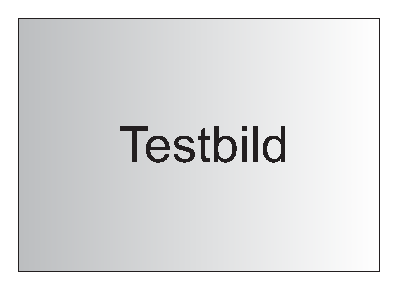
\includegraphics[scale=0.8]{bilder/testbild}\label{fig_testbild2_a}
    }
    \hspace{1.5cm}%
    \subfigure[testbild2b]
         {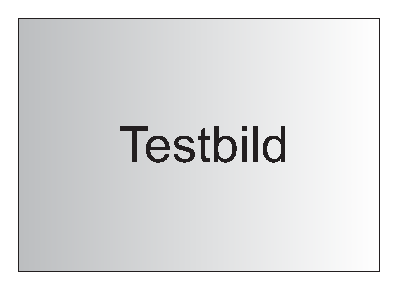
\includegraphics[scale=0.8]{bilder/testbild}\label{fig_testbild2_b}
    }\\
    \subfigure[testbild2c]
          {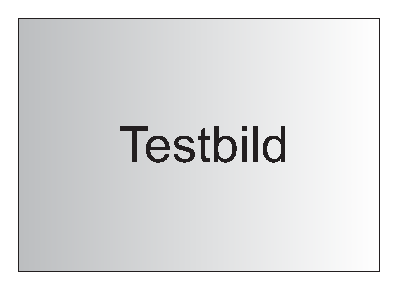
\includegraphics[scale=0.8]{bilder/testbild}\label{fig_testbild2_c}
    }
    \hspace{1.5cm}%
    \subfigure[testbild2d]
         {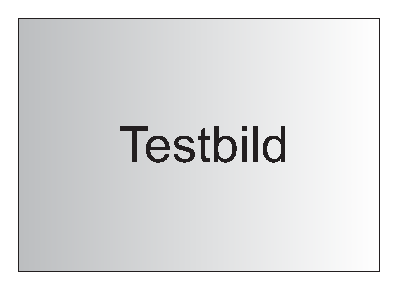
\includegraphics[scale=0.8]{bilder/testbild}\label{fig_testbild2_d}
    }\\
    \caption[Weitere Testbilder]{Weitere Testbilder}
        \label{fig_testbild2}
    \end{figure}

Er presste sich ganz eng an die Wand hinter ihm und hoffte, der
Verfolger würde ihn übersehen, als plötzlich neben ihm mit kaum
wahrnehmbarem Quietschen eine Tür im nächtlichen Wind hin und her
schwang. Könnte dieses der flehentlich herbeigesehnte Ausweg aus
seinem Dilemma sein? Langsam bewegte er sich auf die offene Tür
zu, immer dicht an die Mauer gepresst. Würde diese Tür seine
Rettung werden? Er hörte leise Schritte hinter sich. Das bedeutete
nichts Gutes. Wer würde ihm schon folgen, spät in der Nacht und
dazu noch in dieser engen Gasse mitten im übel beleumundeten
Hafenviertel? Gerade jetzt, wo er das Ding seines Lebens gedreht
hatte und mit der Beute verschwinden wollte! Hatte einer seiner
zahllosen Kollegen dieselbe Idee gehabt, ihn beobachtet und
abgewartet, um ihn nun um die Früchte seiner Arbeit zu
erleichtern? Oder gehörten die Schritte hinter ihm zu einem der
unzähligen Gesetzeshüter dieser Stadt, und die stählerne Acht um
seine Handgelenke würde gleich zuschnappen? Er konnte die
Aufforderung stehen zu bleiben schon hören. Gehetzt sah er sich
um. Plötzlich erblickte er den schmalen Durchgang. Blitzartig
drehte er sich nach rechts und verschwand zwischen den beiden
Gebäuden.

Er hörte \enquote{leise Schritte} hinter sich. Das bedeutete
nichts Gutes. Wer würde ihm schon folgen, spät in der Nacht und
dazu noch in dieser engen Gasse mitten im übel beleumundeten
Hafenviertel? Gerade jetzt, wo er das Ding seines Lebens gedreht
hatte und mit der Beute verschwinden wollte! Hatte einer seiner
zahllosen Kollegen dieselbe Idee gehabt, ihn beobachtet und
abgewartet, um ihn nun um die Früchte seiner Arbeit zu
erleichtern? Oder gehörten die Schritte hinter ihm zu einem der
unzähligen Gesetzeshüter dieser Stadt, und die stählerne Acht um
seine Handgelenke würde gleich zuschnappen? Er konnte die
Aufforderung stehen zu bleiben
schon hören.

Er hörte leise Schritte hinter sich. Das bedeutete nichts Gutes.Wer würde ihm schon folgen,
spät in der Nacht und dazu noch in dieser engen Gasse mitten im übel beleumundeten
Hafenviertel? Gerade jetzt, wo er das Ding seines Lebens gedreht hatte und mit der Beute
verschwinden wollte! Hatte einer seiner zahllosen Kollegen dieselbe Idee gehabt, ihn
beobachtet und abgewartet, um ihn nun um die Früchte seiner Arbeit zu erleichtern?
Oder gehörten die Schritte hinter ihm zu einem der unzähligen Gesetzeshüter dieser
Stadt, und die stählerne Acht um seine Handgelenke würde gleich zuschnappen? Er
konnte die Aufforderung stehen zu bleiben schon hören. Gehetzt sah er sich um. Plötzlich
erblickte er den schmalen Durchgang. Blitzartig drehte er sich nach rechts und verschwand
zwischen den beiden Gebäuden. Beinahe wäre er dabei über den umgestürzten Mülleimer
gefallen, der mitten im Weg lag. Er versuchte, sich in der Dunkelheit seinen Weg zu
ertasten und erstarrte: Anscheinend gab es keinen anderen Ausweg aus diesem kleinen
Hof als den Durchgang, durch den er gekommen war. Die Schritte wurden lauter und
lauter, er sah eine dunkle Gestalt um die Ecke biegen. Fieberhaft irrten seine Augen durch
die nächtliche Dunkelheit und suchten einen Ausweg. War jetzt wirklich alles vorbei,
waren alle Mühe und alle Vorbereitungen umsonst? Er presste sich ganz eng an die Wand
hinter ihm und hoffte, der Verfolger würde ihn übersehen, als plötzlich neben ihm mit
kaum wahrnehmbarem Quietschen eine Tür im nächtlichen Wind hin und her schwang.
Könnte dieses der flehentlich herbeigesehnte Ausweg aus seinem Dilemma sein? Langsam
bewegte er sich auf die offene Tür zu, immer dicht an die Mauer gepresst. Würde diese
Tür seine Rettung werden?

%


\cleardoublepage
%Problems and Solutions
%========================================================================================
% TU Dortmund, Informatik Lehrstuhl VII
%========================================================================================

\chapter{Probleme und L{\"o}sungen}
\label{Probleme_und_Loesungen}
%
Gehetzt sah er sich um. Plötzlich erblickte er den schmalen
Durchgang. Blitzartig drehte er sich nach rechts und verschwand
zwischen den beiden Gebäuden. Beinahe wäre er dabei über den
umgestürzten Mülleimer gefallen, der mitten im Weg lag. Er
versuchte, sich in der Dunkelheit seinen Weg zu ertasten und
erstarrte: Anscheinend gab es keinen anderen Ausweg aus diesem
kleinen Hof als den Durchgang, durch den er gekommen war.

\section{Probleme und L{\"o}sungen - Unterkapitel 1}
\label{Probleme_und_Loesungen_-_Unterkapitel_1}
%
    \begin{algorithm}[t]
    \centering
    \caption[Ein Algorithmus]{Algorithmus} \label{algo_1}
    \begin{algorithmic}
    \REQUIRE Wert $x :=3$
    \ENSURE Wert für $y$
    \STATE $z = 2$
    \WHILE{$(z < 10)$}
    \STATE $x = x + z$
    \FOR{$(1 \leq a \leq z-1)$}
    \STATE $z = z + 1$
    \ENDFOR
    \ENDWHILE
    \end{algorithmic}
    \end{algorithm}


Er hörte \enquote{leise Schritte} hinter sich. Das bedeutete
nichts Gutes. Wer würde ihm schon folgen, spät in der Nacht und
dazu noch in dieser engen Gasse mitten im übel beleumundeten
Hafenviertel? Gerade jetzt, wo er das Ding seines Lebens gedreht
hatte und mit der Beute verschwinden wollte! Hatte einer seiner
zahllosen Kollegen dieselbe Idee gehabt, ihn beobachtet und
abgewartet, um ihn nun um die Früchte seiner Arbeit zu
erleichtern? Oder gehörten die Schritte hinter ihm zu einem der
unzähligen Gesetzeshüter dieser Stadt, und die stählerne Acht um
seine Handgelenke würde gleich zuschnappen? Er konnte die
Aufforderung stehen zu bleiben
schon hören.

Gehetzt sah er sich um. Plötzlich erblickte er den schmalen
Durchgang. Blitzartig drehte er sich nach rechts und verschwand
zwischen den beiden Gebäuden. Beinahe wäre er dabei über den
umgestürzten Mülleimer gefallen, der mitten im Weg lag. Er
versuchte, sich in der Dunkelheit seinen Weg zu ertasten und
erstarrte: Anscheinend gab es keinen anderen Ausweg aus diesem
kleinen Hof als den Durchgang, durch den er gekommen war. Die
Schritte wurden lauter und lauter, er sah eine dunkle Gestalt um
die Ecke biegen. Fieberhaft irrten seine Augen durch die
nächtliche Dunkelheit und suchten einen Ausweg. War jetzt wirklich
alles vorbei, waren alle Mühe und alle Vorbereitungen umsonst?

Er presste sich ganz eng an die Wand hinter ihm und hoffte, der
Verfolger würde ihn übersehen, als plötzlich neben ihm mit kaum
wahrnehmbarem Quietschen eine Tür im nächtlichen Wind hin und her
schwang. Könnte dieses der flehentlich herbeigesehnte Ausweg aus
seinem Dilemma sein? Langsam bewegte er sich auf die offene Tür
zu, immer dicht an die Mauer gepresst. Würde diese Tür seine
Rettung werden? Er hörte leise Schritte hinter sich. Das bedeutete
nichts Gutes. Wer würde ihm schon folgen, spät in der Nacht und
dazu noch in dieser engen Gasse mitten im übel beleumundeten
Hafenviertel? Gerade jetzt, wo er das Ding seines Lebens gedreht
hatte und mit der Beute verschwinden wollte! Hatte einer seiner
zahllosen Kollegen dieselbe Idee gehabt, ihn beobachtet und
abgewartet, um ihn nun um die Früchte seiner Arbeit zu
erleichtern? Oder gehörten die Schritte hinter ihm zu einem der
unzähligen Gesetzeshüter dieser Stadt, und die stählerne Acht um
seine Handgelenke würde gleich zuschnappen? Er konnte die
Aufforderung stehen zu bleiben schon hören. Gehetzt sah er sich
um. Plötzlich erblickte er den schmalen Durchgang. Blitzartig
drehte er sich nach rechts und verschwand zwischen den beiden
Gebäuden.


%\begin{lstlisting}[style=C++, caption=Beispielcode]{Name}
%#include <stdio.h>
%#include <stdlib.h>

%int main() {

%    int counter = 100;
%    for(int i = 1; i < 100; i++){
%        if(counter > i) printf("Hallo");
%        counter--;
%    }
%}

%return 0;
%\end{lstlisting}





\section{Probleme und L{\"o}sungen - Unterkapitel 2}
\label{Probleme_und_Loesungen_-_Unterkapitel_2}
%
\begin{table}[b]
\centering
\begin{tabular}{lrr}
\toprule
\multicolumn{2}{c}{Studium}\\ \cmidrule{1-2}
Fach & Dauer & Einkommen (\euro{})\\
\midrule
Info & 2 & 12,75 \\ \addlinespace
MST & 6 & 8,20 \\ \addlinespace
Informatik & 14 & 10,00\\
\bottomrule
\end{tabular}
\caption{Studium}
\label{table:Studium}
\end{table}
%
Er presste sich ganz eng an die Wand hinter ihm und hoffte, der
Verfolger würde ihn übersehen, als plötzlich neben ihm mit kaum
wahrnehmbarem Quietschen eine Tür im nächtlichen Wind hin und her
schwang. Könnte dieses der flehentlich herbeigesehnte Ausweg aus
seinem Dilemma sein? Langsam bewegte er sich auf die offene Tür
zu, immer dicht an die Mauer gepresst. Würde diese Tür seine
Rettung werden? Er hörte leise Schritte hinter sich. Das bedeutete
nichts Gutes. Wer würde ihm schon folgen, spät in der Nacht und
dazu noch in dieser engen Gasse mitten im übel beleumundeten
Hafenviertel? Gerade jetzt, wo er das Ding seines Lebens gedreht
hatte und mit der Beute verschwinden wollte! Hatte einer seiner
zahllosen Kollegen dieselbe Idee gehabt, ihn beobachtet und
abgewartet, um ihn nun um die Früchte seiner Arbeit zu
erleichtern? Oder gehörten die Schritte hinter ihm zu einem der
unzähligen Gesetzeshüter dieser Stadt, und die stählerne Acht um
seine Handgelenke würde gleich zuschnappen? Er konnte die
Aufforderung stehen zu bleiben schon hören. Gehetzt sah er sich
um. Plötzlich erblickte er den schmalen Durchgang. Blitzartig
drehte er sich nach rechts und verschwand zwischen den beiden
Gebäuden.

    \begin{figure}[t]
    \centering
    \subfigure[testbild2a]
          {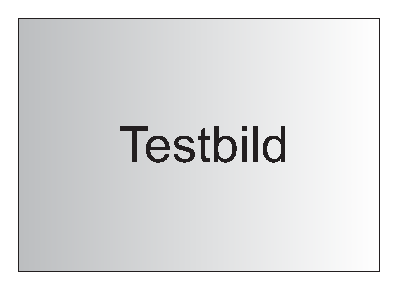
\includegraphics[scale=0.8]{bilder/testbild}\label{fig_testbild2_a}
    }
    \hspace{1.5cm}%
    \subfigure[testbild2b]
         {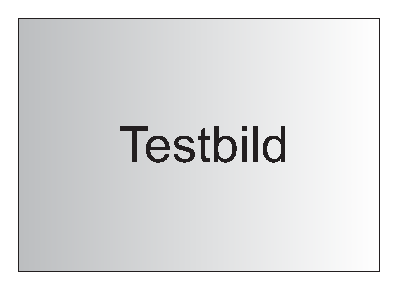
\includegraphics[scale=0.8]{bilder/testbild}\label{fig_testbild2_b}
    }\\
    \subfigure[testbild2c]
          {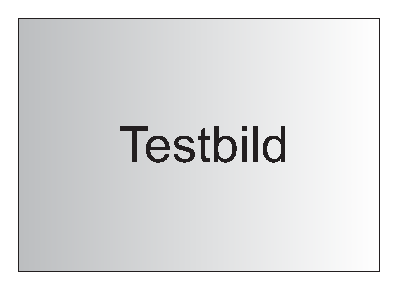
\includegraphics[scale=0.8]{bilder/testbild}\label{fig_testbild2_c}
    }
    \hspace{1.5cm}%
    \subfigure[testbild2d]
         {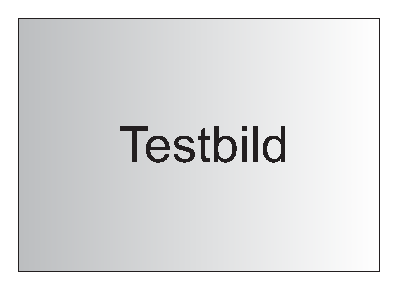
\includegraphics[scale=0.8]{bilder/testbild}\label{fig_testbild2_d}
    }\\
    \caption[Weitere Testbilder]{Weitere Testbilder}
        \label{fig_testbild2}
    \end{figure}

Er presste sich ganz eng an die Wand hinter ihm und hoffte, der
Verfolger würde ihn übersehen, als plötzlich neben ihm mit kaum
wahrnehmbarem Quietschen eine Tür im nächtlichen Wind hin und her
schwang. Könnte dieses der flehentlich herbeigesehnte Ausweg aus
seinem Dilemma sein? Langsam bewegte er sich auf die offene Tür
zu, immer dicht an die Mauer gepresst. Würde diese Tür seine
Rettung werden? Er hörte leise Schritte hinter sich. Das bedeutete
nichts Gutes. Wer würde ihm schon folgen, spät in der Nacht und
dazu noch in dieser engen Gasse mitten im übel beleumundeten
Hafenviertel? Gerade jetzt, wo er das Ding seines Lebens gedreht
hatte und mit der Beute verschwinden wollte! Hatte einer seiner
zahllosen Kollegen dieselbe Idee gehabt, ihn beobachtet und
abgewartet, um ihn nun um die Früchte seiner Arbeit zu
erleichtern? Oder gehörten die Schritte hinter ihm zu einem der
unzähligen Gesetzeshüter dieser Stadt, und die stählerne Acht um
seine Handgelenke würde gleich zuschnappen? Er konnte die
Aufforderung stehen zu bleiben schon hören. Gehetzt sah er sich
um. Plötzlich erblickte er den schmalen Durchgang. Blitzartig
drehte er sich nach rechts und verschwand zwischen den beiden
Gebäuden.

Er hörte \enquote{leise Schritte} hinter sich. Das bedeutete
nichts Gutes. Wer würde ihm schon folgen, spät in der Nacht und
dazu noch in dieser engen Gasse mitten im übel beleumundeten
Hafenviertel? Gerade jetzt, wo er das Ding seines Lebens gedreht
hatte und mit der Beute verschwinden wollte! Hatte einer seiner
zahllosen Kollegen dieselbe Idee gehabt, ihn beobachtet und
abgewartet, um ihn nun um die Früchte seiner Arbeit zu
erleichtern? Oder gehörten die Schritte hinter ihm zu einem der
unzähligen Gesetzeshüter dieser Stadt, und die stählerne Acht um
seine Handgelenke würde gleich zuschnappen? Er konnte die
Aufforderung stehen zu bleiben
schon hören.

Er hörte leise Schritte hinter sich. Das bedeutete nichts Gutes.Wer würde ihm schon folgen,
spät in der Nacht und dazu noch in dieser engen Gasse mitten im übel beleumundeten
Hafenviertel? Gerade jetzt, wo er das Ding seines Lebens gedreht hatte und mit der Beute
verschwinden wollte! Hatte einer seiner zahllosen Kollegen dieselbe Idee gehabt, ihn
beobachtet und abgewartet, um ihn nun um die Früchte seiner Arbeit zu erleichtern?
Oder gehörten die Schritte hinter ihm zu einem der unzähligen Gesetzeshüter dieser
Stadt, und die stählerne Acht um seine Handgelenke würde gleich zuschnappen? Er
konnte die Aufforderung stehen zu bleiben schon hören. Gehetzt sah er sich um. Plötzlich
erblickte er den schmalen Durchgang. Blitzartig drehte er sich nach rechts und verschwand
zwischen den beiden Gebäuden. Beinahe wäre er dabei über den umgestürzten Mülleimer
gefallen, der mitten im Weg lag. Er versuchte, sich in der Dunkelheit seinen Weg zu
ertasten und erstarrte: Anscheinend gab es keinen anderen Ausweg aus diesem kleinen
Hof als den Durchgang, durch den er gekommen war. Die Schritte wurden lauter und
lauter, er sah eine dunkle Gestalt um die Ecke biegen. Fieberhaft irrten seine Augen durch
die nächtliche Dunkelheit und suchten einen Ausweg. War jetzt wirklich alles vorbei,
waren alle Mühe und alle Vorbereitungen umsonst? Er presste sich ganz eng an die Wand
hinter ihm und hoffte, der Verfolger würde ihn übersehen, als plötzlich neben ihm mit
kaum wahrnehmbarem Quietschen eine Tür im nächtlichen Wind hin und her schwang.
Könnte dieses der flehentlich herbeigesehnte Ausweg aus seinem Dilemma sein? Langsam
bewegte er sich auf die offene Tür zu, immer dicht an die Mauer gepresst. Würde diese
Tür seine Rettung werden?

%


%% ----------------------------------------------------------------------
%
%        Vorlage für Abschlussarbeiten am Lehrstuhl Informatik XII
%
%                   http://ls12-www.cs.uni-dortmund.de
%
%   Für Fragen und Anregungen zur Vorlage: info@ls12.cs.uni-dortmund.de
%
%   Stand: 03.09.2013
%
% ----------------------------------------------------------------------

\RequirePackage{ifthen}

\newcommand \type{Fachprojekt Report}
\newcommand \Autor{Lukas B{\"u}nger \\ Thilaksan Kodeeswaran\\ Dilsan Mahadeva}
\newcommand \submissiondate{30.09.2020}
\newcommand \thesistitle{Interactive Real-Time Gaming}
\newcommand \firstsupervisor{Prof.~Dr. Jian-Jia Chen}
\newcommand \secondsupervisor{M.Sc. Junjie Shi}
\newcommand \ErstLehrstuhl{Lehrstuhl Informatik 12 (Eingebettete Systeme) \\ \url{http://ls12-www.cs.tu-dortmund.de}}
\newcommand \ZweitLehrstuhl{}

\RequirePackage{ifpdf} \ifpdf
  \pdfoutput=1
  \pdftrue
  \message{pdfLaTeX}
  \documentclass[pdftex,11pt,a4paper,twoside,ngerman]{scrbook}
  \usepackage{float}
  \usepackage[pdftex]{thumbpdf}
  \usepackage[pdftex]{graphicx}
  \usepackage[pdftex]{hyperref}
  \usepackage{pdfpages}
  \pdfoutput=1
  \pdfcompresslevel=9
  \DeclareGraphicsExtensions{.pdf,.jpg,.png}
\else
  \pdffalse
  \message{LaTeX}
  \documentclass[dvips,11pt,a4paper,twoside,ngerman]{scrbook}
  \usepackage{float}
  \usepackage{graphicx}
  \usepackage{epsf}
  \usepackage[dvips]{hyperref}
  \DeclareGraphicsExtensions{.eps}
\fi

% Informationen fuer pdf-File festlegen
\hypersetup
{
    pdfauthor = {\Autor},
    pdftitle = {\thesistitle},
    pdfsubject = {\type, TU Dortmund, Fakult{\"a}t f{\"u}r Informatik},
    pdfproducer = {LaTeX},
    pdfview = FitV,
    pdfstartview = FitV,
    pdfhighlight = /I,
    pdfborder = 0 0 0,
    colorlinks = false,
    bookmarksopen,
    bookmarksopenlevel = 1,
    bookmarksnumbered = false,
    plainpages = false
}%

% -------------------------------------------------------------------
% Seitenformat anpassen
\usepackage[a4paper,left=3.5cm,right=2.5cm,bottom=3.5cm,top=3cm]{geometry}
\setlength{\headheight}{15pt}

% -------------------------------------------------------------------
% Grafikpakete einbinden
\usepackage{amsmath,amssymb}
\usepackage{flafter}
\usepackage{subfigure}

% -------------------------------------------------------------------
\usepackage{ifthen}

% -------------------------------------------------------------------
\usepackage[absolute,overlay]{textpos}
\setlength{\TPHorizModule}{1mm}
\setlength{\TPVertModule}{\TPHorizModule}
\textblockorigin{0mm}{0mm}
\usepackage{fix-cm}
\usepackage{setspace}
\usepackage{scrhack}

% -------------------------------------------------------------------
% Korrekte Darstellung der Umlaute
% \usepackage[german,ngerman]{babel}
% \usepackage[utf8]{inputenc}
% \usepackage[T1]{fontenc}
% \usepackage{ae,aecompl}

% -------------------------------------------------------------------
% Bibtex deutsch
%\usepackage[numbers,sort,square]{natbib}
%\usepackage{bibgerm}

% -------------------------------------------------------------------
% Anführungszeichen
\usepackage[babel,german=quotes]{csquotes}

% -------------------------------------------------------------------
% URLs
\usepackage{url}

% -------------------------------------------------------------------
% Caption anpassen
\usepackage[margin=0pt,font=small,labelfont=bf]{caption}

% -------------------------------------------------------------------
% Erweitere Tabellen
\usepackage{booktabs}

% -------------------------------------------------------------------
% Eurosymbol
\usepackage{eurosym}

% -------------------------------------------------------------------
% Zeilenabstand einstellen
\renewcommand{\baselinestretch}{1.25}
% Floating-Umgebungen anpassen
\renewcommand{\topfraction}{0.9}
\renewcommand{\bottomfraction}{0.8}

% -------------------------------------------------------------------
% Keine einzelnen Zeilen beim Anfang eines Abschnitts ("Schusterjungen")
\clubpenalty = 10000
% Keine einzelnen Zeilen am Ende eines Abschnitts ("Hurenkinder")
\widowpenalty = 10000 \displaywidowpenalty = 10000
\parindent=0cm

% -------------------------------------------------------------------
% Kopfzeile hinzufuegen
\usepackage{fancyhdr}
\usepackage{extramarks}

\pagestyle{fancy}
\renewcommand{\chaptermark}[1]{\markboth{#1}{}}
\renewcommand{\sectionmark}[1]{\markright{#1}{}}

\fancyhf{}
\fancyhead[LE,RO]{\thepage}
\fancyhead[RE]{\textit{\nouppercase{\leftmark}}}
\fancyhead[LO]{\textit{\nouppercase{\rightmark}}}

\fancypagestyle{plain}{ %
\fancyhf{} % remove everything
\renewcommand{\headrulewidth}{0pt} % remove lines as well
\renewcommand{\footrulewidth}{0pt}} \pagestyle{headings}

% -------------------------------------------------------------------
% Eigene Farben definieren
\usepackage{color}
\definecolor{TUGreen}{rgb}{0.517,0.721,0.094}
\definecolor{TUOrange}{rgb}{1.0,0.7176,0.0}
\definecolor{BrightGray}{gray}{0.9}
\definecolor{DarkGray}{gray}{0.2}
\definecolor{white}{rgb}{1,1,1}
\definecolor{black}{rgb}{0,0,0}
\definecolor{red}{rgb}{1,0,0}

% -------------------------------------------------------------------
% Programm-Listings einbinden und formatieren
\usepackage{listings}

\lstdefinestyle{C++}
{
language=C++,
backgroundcolor=\color{BrightGray},
keywordstyle=\tt\bfseries,  %\color{TUGreen}\bfseries,
commentstyle=\color{DarkGray},
stringstyle=\color{red},
showstringspaces=false,
basicstyle=\small\color{black},
numbers=left,
captionpos=b,
tabsize=4,
breaklines=true
}

% -------------------------------------------------------------------
% Algorithmen
\usepackage[plain,chapter]{algorithm}
\usepackage{algorithmic}

\usepackage{enumerate}

% -------------------------------------------------------------------
% Algorithmen anpassen
\renewcommand{\algorithmicrequire}{\textit{Eingabe:}}
\renewcommand{\algorithmicensure}{\textit{Ausgabe:}}
\floatname{algorithm}{Algorithmus}
\renewcommand{\listalgorithmname}{Algorithmenverzeichnis}
\renewcommand{\algorithmiccomment}[1]{\color{grau}{// #1}}

% -------------------------------------------------------------------
% Theorem-Umgebungen
\usepackage[amsmath,thmmarks]{ntheorem}
\theoremseparator{.}
\theoremstyle{change}
\newtheorem{theorem}{Theorem}[section]
\newtheorem{satz}[theorem]{Satz}
\newtheorem{lemma}[theorem]{Lemma}
\newtheorem{korollar}[theorem]{Korollar}
\newtheorem{proposition}[theorem]{Proposition}
% Ohne Numerierung
\theoremstyle{nonumberplain}
\renewtheorem{theorem*}{Theorem}
\renewtheorem{satz*}{Satz}
\renewtheorem{lemma*}{Lemma}
\renewtheorem{korollar*}{Korollar}
\renewtheorem{proposition*}{Proposition}
% Definitionen mit \upshape
\theorembodyfont{\upshape}
\theoremstyle{change}
\newtheorem{definition}[theorem]{Definition}
\theoremstyle{nonumberplain}
\renewtheorem{definition*}{Definition}
% Kursive Schrift
\theoremheaderfont{\itshape}
\newtheorem{notation}{Notation}
\newtheorem{konvention}{Konvention}
\newtheorem{bezeichnung}{Bezeichnung}
\theoremsymbol{\ensuremath{\Box}}
\newtheorem{beweis}{Beweis}
\theoremsymbol{}
\theoremstyle{change}
\theoremheaderfont{\bfseries}
\newtheorem{bemerkung}[theorem]{Bemerkung}
\newtheorem{beobachtung}[theorem]{Beobachtung}
\newtheorem{beispiel}[theorem]{Beispiel}
\newtheorem{problem}{Problem}
\theoremstyle{nonumberplain}
\renewtheorem{bemerkung*}{Bemerkung}
\renewtheorem{beispiel*}{Beispiel}
\renewtheorem{problem*}{Problem}

% Algorithmen anpassen %
\renewcommand{\algorithmicrequire}{\textit{Eingabe:}}
\renewcommand{\algorithmicensure}{\textit{Ausgabe:}}
\floatname{algorithm}{Algorithmus}
\renewcommand{\listalgorithmname}{Algorithmenverzeichnis}
\renewcommand{\algorithmiccomment}[1]{\color{grau}{// #1}}

% Zeilenabstand einstellen %
\renewcommand{\baselinestretch}{1.25}
% Floating-Umgebungen anpassen %
\renewcommand{\topfraction}{0.9}
\renewcommand{\bottomfraction}{0.8}
% Abkuerzungen richtig formatieren %
\usepackage{xspace}
\newcommand{\vgl}{vgl.\@\xspace} 
\newcommand{\zB}{z.\nolinebreak[4]\hspace{0.125em}\nolinebreak[4]B.\@\xspace}
\newcommand{\bzw}{bzw.\@\xspace}
\newcommand{\dahe}{d.\nolinebreak[4]\hspace{0.125em}h.\nolinebreak[4]\@\xspace}
\newcommand{\etc}{etc.\@\xspace}
\newcommand{\evtl}{evtl.\@\xspace}
\newcommand{\ggf}{ggf.\@\xspace}
\newcommand{\bzgl}{bzgl.\@\xspace}
\newcommand{\so}{s.\nolinebreak[4]\hspace{0.125em}\nolinebreak[4]o.\@\xspace}
\newcommand{\iA}{i.\nolinebreak[4]\hspace{0.125em}\nolinebreak[4]A.\@\xspace}
\newcommand{\sa}{s.\nolinebreak[4]\hspace{0.125em}\nolinebreak[4]a.\@\xspace}
\newcommand{\su}{s.\nolinebreak[4]\hspace{0.125em}\nolinebreak[4]u.\@\xspace}
\newcommand{\ua}{u.\nolinebreak[4]\hspace{0.125em}\nolinebreak[4]a.\@\xspace}
\newcommand{\og}{o.\nolinebreak[4]\hspace{0.125em}\nolinebreak[4]g.\@\xspace}
\newcommand{\oBdA}{o.\nolinebreak[4]\hspace{0.125em}\nolinebreak[4]B.\nolinebreak[4]\hspace{0.125em}d.\nolinebreak[4]\hspace{0.125em}A.\@\xspace}
\newcommand{\OBdA}{O.\nolinebreak[4]\hspace{0.125em}\nolinebreak[4]B.\nolinebreak[4]\hspace{0.125em}d.\nolinebreak[4]\hspace{0.125em}A.\@\xspace}

% Leere Seite ohne Seitennummer, naechste Seite rechts
\newcommand{\blankpage}{
 \clearpage{\pagestyle{empty}\cleardoublepage}
}


\begin{document}

% Erklaerung -----------------------------------------------------------
%
\thispagestyle{myheadings}
\markboth{}{ERKLÄRUNG}
% ----------------------------------------------------------------------
%
%        Vorlage für Abschlussarbeiten am Lehrstuhl Informatik XII
%
%                   http://ls12-www.cs.uni-dortmund.de
%
%   Für Fragen und Anregungen zur Vorlage: info@ls12.cs.uni-dortmund.de
%
%   Stand: 03.09.2013
%
% ----------------------------------------------------------------------

\RequirePackage{ifthen}

\newcommand \type{Fachprojekt Report}
\newcommand \Autor{Lukas B{\"u}nger \\ Thilaksan Kodeeswaran\\ Dilsan Mahadeva}
\newcommand \submissiondate{30.09.2020}
\newcommand \thesistitle{Interactive Real-Time Gaming}
\newcommand \firstsupervisor{Prof.~Dr. Jian-Jia Chen}
\newcommand \secondsupervisor{M.Sc. Junjie Shi}
\newcommand \ErstLehrstuhl{Lehrstuhl Informatik 12 (Eingebettete Systeme) \\ \url{http://ls12-www.cs.tu-dortmund.de}}
\newcommand \ZweitLehrstuhl{}

\RequirePackage{ifpdf} \ifpdf
  \pdfoutput=1
  \pdftrue
  \message{pdfLaTeX}
  \documentclass[pdftex,11pt,a4paper,twoside,ngerman]{scrbook}
  \usepackage{float}
  \usepackage[pdftex]{thumbpdf}
  \usepackage[pdftex]{graphicx}
  \usepackage[pdftex]{hyperref}
  \usepackage{pdfpages}
  \pdfoutput=1
  \pdfcompresslevel=9
  \DeclareGraphicsExtensions{.pdf,.jpg,.png}
\else
  \pdffalse
  \message{LaTeX}
  \documentclass[dvips,11pt,a4paper,twoside,ngerman]{scrbook}
  \usepackage{float}
  \usepackage{graphicx}
  \usepackage{epsf}
  \usepackage[dvips]{hyperref}
  \DeclareGraphicsExtensions{.eps}
\fi

% Informationen fuer pdf-File festlegen
\hypersetup
{
    pdfauthor = {\Autor},
    pdftitle = {\thesistitle},
    pdfsubject = {\type, TU Dortmund, Fakult{\"a}t f{\"u}r Informatik},
    pdfproducer = {LaTeX},
    pdfview = FitV,
    pdfstartview = FitV,
    pdfhighlight = /I,
    pdfborder = 0 0 0,
    colorlinks = false,
    bookmarksopen,
    bookmarksopenlevel = 1,
    bookmarksnumbered = false,
    plainpages = false
}%

% -------------------------------------------------------------------
% Seitenformat anpassen
\usepackage[a4paper,left=3.5cm,right=2.5cm,bottom=3.5cm,top=3cm]{geometry}
\setlength{\headheight}{15pt}

% -------------------------------------------------------------------
% Grafikpakete einbinden
\usepackage{amsmath,amssymb}
\usepackage{flafter}
\usepackage{subfigure}

% -------------------------------------------------------------------
\usepackage{ifthen}

% -------------------------------------------------------------------
\usepackage[absolute,overlay]{textpos}
\setlength{\TPHorizModule}{1mm}
\setlength{\TPVertModule}{\TPHorizModule}
\textblockorigin{0mm}{0mm}
\usepackage{fix-cm}
\usepackage{setspace}
\usepackage{scrhack}

% -------------------------------------------------------------------
% Korrekte Darstellung der Umlaute
% \usepackage[german,ngerman]{babel}
% \usepackage[utf8]{inputenc}
% \usepackage[T1]{fontenc}
% \usepackage{ae,aecompl}

% -------------------------------------------------------------------
% Bibtex deutsch
%\usepackage[numbers,sort,square]{natbib}
%\usepackage{bibgerm}

% -------------------------------------------------------------------
% Anführungszeichen
\usepackage[babel,german=quotes]{csquotes}

% -------------------------------------------------------------------
% URLs
\usepackage{url}

% -------------------------------------------------------------------
% Caption anpassen
\usepackage[margin=0pt,font=small,labelfont=bf]{caption}

% -------------------------------------------------------------------
% Erweitere Tabellen
\usepackage{booktabs}

% -------------------------------------------------------------------
% Eurosymbol
\usepackage{eurosym}

% -------------------------------------------------------------------
% Zeilenabstand einstellen
\renewcommand{\baselinestretch}{1.25}
% Floating-Umgebungen anpassen
\renewcommand{\topfraction}{0.9}
\renewcommand{\bottomfraction}{0.8}

% -------------------------------------------------------------------
% Keine einzelnen Zeilen beim Anfang eines Abschnitts ("Schusterjungen")
\clubpenalty = 10000
% Keine einzelnen Zeilen am Ende eines Abschnitts ("Hurenkinder")
\widowpenalty = 10000 \displaywidowpenalty = 10000
\parindent=0cm

% -------------------------------------------------------------------
% Kopfzeile hinzufuegen
\usepackage{fancyhdr}
\usepackage{extramarks}

\pagestyle{fancy}
\renewcommand{\chaptermark}[1]{\markboth{#1}{}}
\renewcommand{\sectionmark}[1]{\markright{#1}{}}

\fancyhf{}
\fancyhead[LE,RO]{\thepage}
\fancyhead[RE]{\textit{\nouppercase{\leftmark}}}
\fancyhead[LO]{\textit{\nouppercase{\rightmark}}}

\fancypagestyle{plain}{ %
\fancyhf{} % remove everything
\renewcommand{\headrulewidth}{0pt} % remove lines as well
\renewcommand{\footrulewidth}{0pt}} \pagestyle{headings}

% -------------------------------------------------------------------
% Eigene Farben definieren
\usepackage{color}
\definecolor{TUGreen}{rgb}{0.517,0.721,0.094}
\definecolor{TUOrange}{rgb}{1.0,0.7176,0.0}
\definecolor{BrightGray}{gray}{0.9}
\definecolor{DarkGray}{gray}{0.2}
\definecolor{white}{rgb}{1,1,1}
\definecolor{black}{rgb}{0,0,0}
\definecolor{red}{rgb}{1,0,0}

% -------------------------------------------------------------------
% Programm-Listings einbinden und formatieren
\usepackage{listings}

\lstdefinestyle{C++}
{
language=C++,
backgroundcolor=\color{BrightGray},
keywordstyle=\tt\bfseries,  %\color{TUGreen}\bfseries,
commentstyle=\color{DarkGray},
stringstyle=\color{red},
showstringspaces=false,
basicstyle=\small\color{black},
numbers=left,
captionpos=b,
tabsize=4,
breaklines=true
}

% -------------------------------------------------------------------
% Algorithmen
\usepackage[plain,chapter]{algorithm}
\usepackage{algorithmic}

\usepackage{enumerate}

% -------------------------------------------------------------------
% Algorithmen anpassen
\renewcommand{\algorithmicrequire}{\textit{Eingabe:}}
\renewcommand{\algorithmicensure}{\textit{Ausgabe:}}
\floatname{algorithm}{Algorithmus}
\renewcommand{\listalgorithmname}{Algorithmenverzeichnis}
\renewcommand{\algorithmiccomment}[1]{\color{grau}{// #1}}

% -------------------------------------------------------------------
% Theorem-Umgebungen
\usepackage[amsmath,thmmarks]{ntheorem}
\theoremseparator{.}
\theoremstyle{change}
\newtheorem{theorem}{Theorem}[section]
\newtheorem{satz}[theorem]{Satz}
\newtheorem{lemma}[theorem]{Lemma}
\newtheorem{korollar}[theorem]{Korollar}
\newtheorem{proposition}[theorem]{Proposition}
% Ohne Numerierung
\theoremstyle{nonumberplain}
\renewtheorem{theorem*}{Theorem}
\renewtheorem{satz*}{Satz}
\renewtheorem{lemma*}{Lemma}
\renewtheorem{korollar*}{Korollar}
\renewtheorem{proposition*}{Proposition}
% Definitionen mit \upshape
\theorembodyfont{\upshape}
\theoremstyle{change}
\newtheorem{definition}[theorem]{Definition}
\theoremstyle{nonumberplain}
\renewtheorem{definition*}{Definition}
% Kursive Schrift
\theoremheaderfont{\itshape}
\newtheorem{notation}{Notation}
\newtheorem{konvention}{Konvention}
\newtheorem{bezeichnung}{Bezeichnung}
\theoremsymbol{\ensuremath{\Box}}
\newtheorem{beweis}{Beweis}
\theoremsymbol{}
\theoremstyle{change}
\theoremheaderfont{\bfseries}
\newtheorem{bemerkung}[theorem]{Bemerkung}
\newtheorem{beobachtung}[theorem]{Beobachtung}
\newtheorem{beispiel}[theorem]{Beispiel}
\newtheorem{problem}{Problem}
\theoremstyle{nonumberplain}
\renewtheorem{bemerkung*}{Bemerkung}
\renewtheorem{beispiel*}{Beispiel}
\renewtheorem{problem*}{Problem}

% Algorithmen anpassen %
\renewcommand{\algorithmicrequire}{\textit{Eingabe:}}
\renewcommand{\algorithmicensure}{\textit{Ausgabe:}}
\floatname{algorithm}{Algorithmus}
\renewcommand{\listalgorithmname}{Algorithmenverzeichnis}
\renewcommand{\algorithmiccomment}[1]{\color{grau}{// #1}}

% Zeilenabstand einstellen %
\renewcommand{\baselinestretch}{1.25}
% Floating-Umgebungen anpassen %
\renewcommand{\topfraction}{0.9}
\renewcommand{\bottomfraction}{0.8}
% Abkuerzungen richtig formatieren %
\usepackage{xspace}
\newcommand{\vgl}{vgl.\@\xspace} 
\newcommand{\zB}{z.\nolinebreak[4]\hspace{0.125em}\nolinebreak[4]B.\@\xspace}
\newcommand{\bzw}{bzw.\@\xspace}
\newcommand{\dahe}{d.\nolinebreak[4]\hspace{0.125em}h.\nolinebreak[4]\@\xspace}
\newcommand{\etc}{etc.\@\xspace}
\newcommand{\evtl}{evtl.\@\xspace}
\newcommand{\ggf}{ggf.\@\xspace}
\newcommand{\bzgl}{bzgl.\@\xspace}
\newcommand{\so}{s.\nolinebreak[4]\hspace{0.125em}\nolinebreak[4]o.\@\xspace}
\newcommand{\iA}{i.\nolinebreak[4]\hspace{0.125em}\nolinebreak[4]A.\@\xspace}
\newcommand{\sa}{s.\nolinebreak[4]\hspace{0.125em}\nolinebreak[4]a.\@\xspace}
\newcommand{\su}{s.\nolinebreak[4]\hspace{0.125em}\nolinebreak[4]u.\@\xspace}
\newcommand{\ua}{u.\nolinebreak[4]\hspace{0.125em}\nolinebreak[4]a.\@\xspace}
\newcommand{\og}{o.\nolinebreak[4]\hspace{0.125em}\nolinebreak[4]g.\@\xspace}
\newcommand{\oBdA}{o.\nolinebreak[4]\hspace{0.125em}\nolinebreak[4]B.\nolinebreak[4]\hspace{0.125em}d.\nolinebreak[4]\hspace{0.125em}A.\@\xspace}
\newcommand{\OBdA}{O.\nolinebreak[4]\hspace{0.125em}\nolinebreak[4]B.\nolinebreak[4]\hspace{0.125em}d.\nolinebreak[4]\hspace{0.125em}A.\@\xspace}

% Leere Seite ohne Seitennummer, naechste Seite rechts
\newcommand{\blankpage}{
 \clearpage{\pagestyle{empty}\cleardoublepage}
}


\begin{document}

% Erklaerung -----------------------------------------------------------
%
\thispagestyle{myheadings}
\markboth{}{ERKLÄRUNG}
% ----------------------------------------------------------------------
%
%        Vorlage für Abschlussarbeiten am Lehrstuhl Informatik XII
%
%                   http://ls12-www.cs.uni-dortmund.de
%
%   Für Fragen und Anregungen zur Vorlage: info@ls12.cs.uni-dortmund.de
%
%   Stand: 03.09.2013
%
% ----------------------------------------------------------------------

\include{header}

\begin{document}

% Erklaerung -----------------------------------------------------------
%
\thispagestyle{myheadings}
\markboth{}{ERKLÄRUNG}
\include{chapter/erklaerung}

% ----------------------------------------------------------------------

\end{document}


% ----------------------------------------------------------------------

\end{document}


% ----------------------------------------------------------------------

\end{document}

% Anhang ---------------------------------------------------------------
%
\cleardoublepage
\appendix


%========================================================================================
% TU Dortmund, Informatik Lehrstuhl VII
%========================================================================================

\chapter*{Appendix}




% Abbildungsverzeichnis -------------------------------------------------
%
\listoffigures
\addcontentsline{toc}{chapter}{List of Figures }
\cleardoublepage

% Algorithmenverzeichnis ------------------------------------------------
%
\listofalgorithms
\addcontentsline{toc}{chapter}{List of Algorithms}
\cleardoublepage

% Quellcodeverzeichnis --------------------------------------------------
%
\renewcommand{\lstlistlistingname}{List of Source Codes}
\lstlistoflistings
\addcontentsline{toc}{chapter}{List of Source Codes}
\cleardoublepage
% ----------------------------------------------------------------------


%\cleardoublepage
%\addcontentsline{toc}{chapter}{Eidesstattliche Versicherung}
%\include{Eidesstattliche_Versicherung.pdf}
\clearpage
\pagestyle{empty}
\addcontentsline{toc}{chapter}{Eidesstattliche Versicherung}
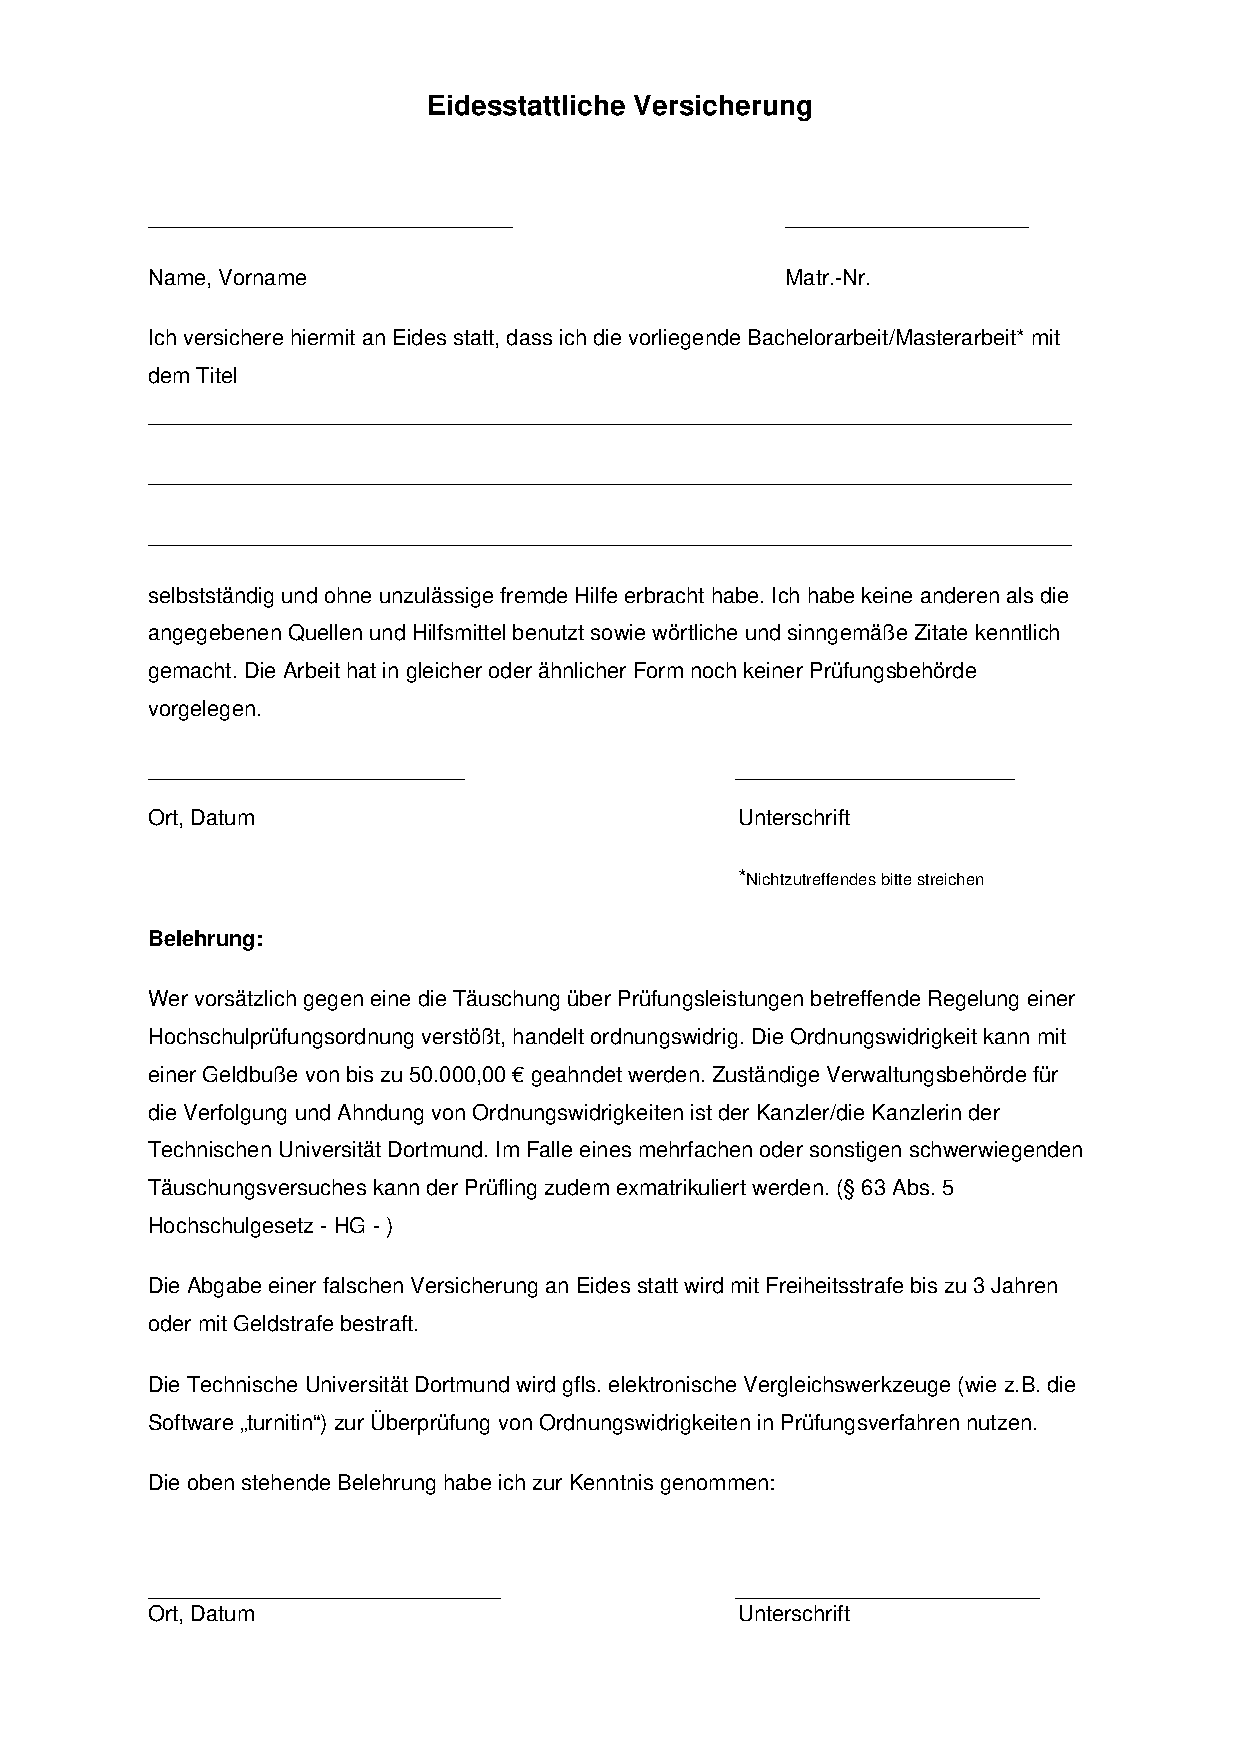
\includegraphics[trim = 20mm 20mm 20mm 10mm, clip,
width=\textwidth]{Eidesstattliche_Versicherung.pdf}


%%========================================================================================
% TU Dortmund, Informatik Lehrstuhl VII
%========================================================================================

\chapter*{Appendix}




\end{document}
